% vim:syntax=tex

\begin{figure*}[t]
    \centering
\begin{subfigure}[t]{.9\textwidth}
    \centerline{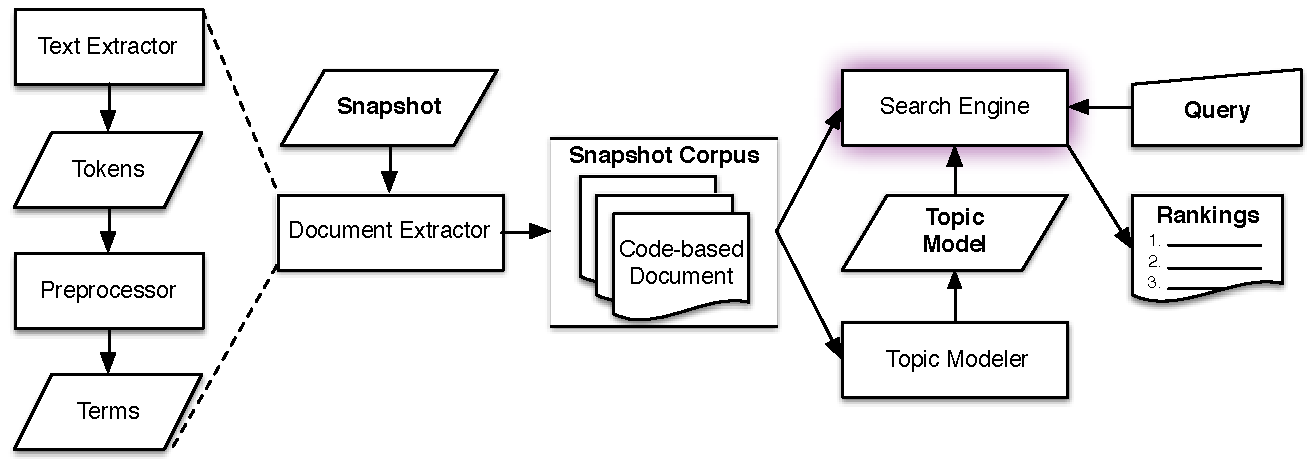
\includegraphics[width=\textwidth]{figures/snapshot-flt}}
    \caption{Feature location using snapshots}
    \label{fig:snapshot}
\end{subfigure}

\begin{subfigure}[b]{.9\textwidth}
    \centerline{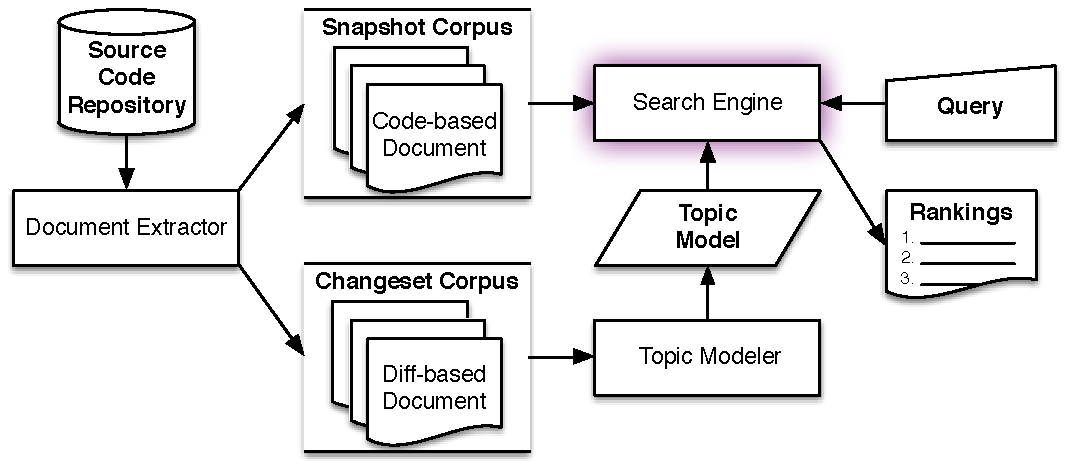
\includegraphics[width=\textwidth]{figures/changeset-flt}}
\caption{Feature location using changesets}
\label{fig:changeset}
\end{subfigure}

\label{fig:flts}
\caption{Two feature location techniques side-by-side}
\end{figure*}


In this section, we review background material of the document extraction and retrieval process
typically used on snapshot-based FLTs,
and review related work on topic modeling and feature location.

\subsection{Document Extraction and Retrieval Process}
\label{sec:snapshot-flt}

We use the following terminology to describe document extraction of source code.
A \textit{word} is the basic unit of discrete data in a software lexicon and is a sequence of letters.
A \textit{token} is a sequence of non-whitespace characters containing one or more words.
An \textit{entity} is a named source element such as a method,
and an \textit{identifier} is a token representing the name of an entity.
\textit{Comments} and \textit{literals} are sequences of tokens delimited by language-specific markers (e.g., /* */ and quotes).
The \textit{document} which corresponds to a class is a sequence of words $d = (w_1, \ldots, w_m)$,
and a \textit{corpus} is a set of documents (i.e., classes) $D = (d_1, \ldots, d_n)$.

The left side of Figure~\ref{fig:snapshot} illustrates the document extraction
process.  A document extractor takes source code as input and produces a corpus
as output.  Each document in the corpus contains the words associated with
a source code entity such as a class or method.  The text extractor is the first
part of the document extractor.  It parses the source code and produces a token
stream for each class.  The preprocessor is the second part of the document
extractor.  It applies a series of transformations to each token and produces
one or more words from the token.
The transformations~\cite{Marcus-etal:2004,Marcus-Menzies:2010}: % that we use are:
\begin{itemize}
    \item {\it Splitting}: separate tokens into constituent words based on
        common coding style conventions (e.g., the use of camel case or
        underscores) and on the presence of non-letters (e.g., punctuation or
        digits)
    \item {\it Normalizing}: replace each upper case letter with the
        corresponding lower case letter
    \item {\it Filtering}: remove common words such as articles (e.g., `an' or
        `the'), programming language keywords, standard library entity names, or
        short words
\end{itemize}

The right side of Figure~\ref{fig:snapshot} illustrates the retrieval process.
The main prerequisite of the retrieval process is to build the search engine.
The search engine is constructed from a topic model trained from a corpus and an
index of that corpus inferred from that model.
This means that an index is no more than each input document's thematic
structure, or inferred topic distribution.

The primary function of the search engine is to rank documents in relation to
the query.  First, the engine must first infer the thematic structure of the
query.  This allows for a pairwise classification of the query to each document
in the index and ranks the documents based on the similarities of their thematic
structures.

\subsection{Latent Dirichlet Allocation}

Latent Dirichlet allocation~\cite{Blei-etal:2003} is a generative topic model.
LDA models each document in a corpus of discrete data as a finite mixture over
a set of topics and models each topic as an infinite mixture over a set of
topic probabilities.  That is, LDA models each document as a probability
distribution indicating the likelihood that it expresses each topic and models
each topic that it infers as a probability distribution indicating the
likelihood of a word from the corpus being assigned to the topic.

Hoffman et al.~\cite{Hoffman-etal:2010} introduce a version of LDA which is
\emph{online}.  Online LDA allows the model to be updated incrementally without
needing to know about the documents prior to model construction.  Zhai and
Boyd-Graber~\cite{Zhai-Boyd-Graber:2013} introduce an extension of LDA in which
the model also does not need to know about the corpus vocabulary prior to
training.


\subsection{Feature Location}

Feature location is the act of identifying the source code entity or entities
that implement a feature~\cite{Rajlich-Wilde:2002}.  Bug localization can be
seen as the process of identifying source code entities that implement an
\emph{unwanted} feature~\cite{Lukins-etal:2010}.

The most closely related work is Rao et al.~\cite{Rao-etal:2013}. Rao et al.\
also target the problem of building topic models, introducing an incremental
framework for bug localization.  Although practical, the approach involves using
an extended topic modeler to allow updating, adding, and removing documents from
the model and index post-hoc.  While the approach is essentially equivalent to
topic modeling in batch, Rao~\cite{Rao:2013} notes that these algorithm
modifications have limitations and thus models may need to be periodically
retrained.

Dit et al.~\cite{Dit-etal:2011} provide a taxonomy and survey of feature
location in source code covering the scope of FLTs.  They identify 89 works
related to feature location in their systematic literature survey and extract
7 dimensions for their taxonomy.  The primary dimension, type of analysis, can
be used for categoization purposes and consists of four categories: dynamic,
static, historical, and textual.

Dynamic FLTs use information from a system's execution, such as stack
traces~\cite{Moreno-etal:2014}.  Static FLTs instead use semantic information
extracted directly from source code, such as method call
graphs~\cite{Saul-etal:2007}.  Historical FLTs use mining software repositories
to extract meaningful information, such as in Cubranic et
al.~\cite{Cubranic-etal:2005}.  Textual FLTs use textual information extracted
from software artifacts, such as source code comments, identifiers, and
literals~\cite{Biggers-etal:2014}. Textual FLTs are the most closely related
category of our work and comprise the remainder of this section.

Currently, developers rely on tools such as \texttt{grep} to find relevant
source code entities. Petrenko et al.~\cite{Petrenko-etal:2008} develop
a \texttt{grep}-based FLT. However, Ko et al.~\cite{Ko-etal:2006} show that
developers fail using this type of searching upwards to 88\% of the time.  Text
retrieval techniques, such as topic modeling, show promise in remedying this
problem~\cite{Marcus-etal:2004}.

Marcus et al~\cite{Marcus-etal:2004} use an FLT based on Latent Semantic
Indexing (LSI)~\cite{Deerwester-etal:1990} to find concepts based on queries
from the user, and modules within the system in comparison to the dependence
graph approach. They found that concepts in the code were able to be identified
with user specified terms and identifiers as well as an easier build process.
LSI-based FLTs have been widely used by many others~\cite{ Poshyvanyk-etal:2006,
Poshyvanyk-Marcus:2007, Liu-etal:2007, Scanniello-Marcus:2011, % Eaddy-etal:2008,
Cubranic-etal:2005}.

Lukins et al.~\cite{Lukins-etal:2008} introduce an FLT based on LDA and find
that it outperforms an LSI-based FLT.  Biggers et al.~\cite{Biggers-etal:2014}
investigate the various configuration parameters for an LDA-based FLT.  Bassett
and Kraft~\cite{Bassett-Kraft:2013} find that using structural term weighting
increases the performance of an LDA-based FLT.

\subsection{Modeling Software Repositories}

Our work is also not the first to investigate ways to employ topic models on
software repositories. Thomas et al.~\cite{Thomas-etal:2011} present a study on
how topics of a software project evolve over time. They present the \emph{Diff}
model, and closely resembles our work. However, their Diff model is much more
coarse-grained and trains a topic model on changesets between two software
snapshots, not changesets between two commits. Additionally, their goal in using
this model is for modeling the evolution of topics, not for feature location.

Finally, Hindle et al.~\cite{Hindle-etal:2009} present a technique that links
requirement documents to code commits using LDA.  They apply LDA to extract
topics from issue reports, requirement documents, and commit messages.  Their
linking process relies on LDA inferencing to derive the topics of unseen
documents.  Our methodology is constructed from this same inferencing concept to
construct an index out of source code entities as they relate to topics learned
from changesets.
